\section{Introduction}

A central concern of modern biology is understanding at the molecular level the chemical and physical mechanisms by which protein and nucleic acid macromolecules  perform essential cellular functions.  The operation of many such macromolecules requires that they work not as isolated molecules in solution but as components of dynamic molecular complexes that self-assemble and change structure and composition as they function.  For more than  two decades, scientists have successfully explored the molecular mechanisms of many such complex and dynamic systems using multi-wavelength single molecule fluorescence methods such as smFRET (single-molecule fluorescence resonance energy transfer) \citep{Roy2008-fo} and multi-wavelength single-molecule colocalization methods (CoSMoS, colocalization single molecule spectroscopy) \citep{Larson2014-os, Van_Oijen2011-ig,Friedman2012-if}.

CoSMoS is a technique to measure the kinetics of dynamic interactions between individual molecules.  The CoSMoS method has been used for elucidating the mechanisms of complex biochemical processes \textit{in vitro}. Examples include cell cycle regulation \citep{Lu2015-eu}, ubiquitination and proteasome-mediated protein degradation \citep{Lu2015-jq}, DNA replication \citep{Geertsema2014-bt,Ticau2015-ib}, transcription \citep{Zhang2012-no,Friedman2012-if,Friedman2013-sf}, micro-RNA regulation \citep{Salomon2015-kq}, pre-mRNA splicing \citep{Shcherbakova2013-bi, Krishnan2013-fy, Warnasooriya2014-ls}, ribosome assembly \citep{Kim2014-zc}, translation \citep{Wang2015-tt,Tsai2014-mi,OLeary2013-wo}, signal recognition particle-nascent protein interaction \citep{Noriega2014-vj}, and cytoskeletal regulation \citep{Smith2013-qj,Breitsprecher2012-mj}. 

\FIG{cosmos_experiment}A illustrates an example CoSMoS experiment to measure the interaction kinetics of RNA polymerase II molecules with DNA. In the experiment \citep{Rosen2020-zn}, we first measured the locations of individual DNA molecules (the ``targets'') tethered to the surface of an observation chamber at low density. Next, a cell extract solution containing fluorescent RNA polymerase II molecules (the ``binders'') was added to the solution over the surface and the chamber surface was imaged by total internal reflection fluorescence (TIRF) microscopy. When the binder molecules are freely diffusing in solution, they are not visible in TIRF. In contrast, when bound to a target, a single binder molecule is detected as a discrete fluorescent spot colocalized with the target position \citep{Friedman2006-kb, Friedman2015-nx}.

Effective data analysis is a major challenge in the use of the CoSMoS technique. The basic goal is to acquire information at each time point about whether a binder molecule fluorescence spot is observed at the image position of a target molecule (e.g., whether a colocalized green-dye-labeled RNA polymerase II is observed at the surface location of a blue-dye-labeled DNA spot in \FIG{cosmos_experiment}B). Although CoSMoS images are conceptually simple -- they consist only of diffraction-limited fluorescent spots collected in several wavelength channels -- efficient analysis of the images is inherently challenging. The number of photons emitted by a single fluorophore is limited by fluorophore photobleaching. Consequently, it is desirable to work at the lowest feasible excitation power in order to maximize the duration of experimental recordings and to efficiently capture relevant reaction events. Achieving higher time resolution divides the number of emitted photons between a larger number of images, so that photon shot noise ordinarily dominates the data statistics. Furthermore, the required concentrations of binder molecules can sometimes create significant background noise \citep{Peng2018-ge, Van_Oijen2011-ig}, even with zero-mode waveguide instruments \citep{Chen2014-jd}. These technical difficulties frequently result in CoSMoS images that have low signal-to-noise ratios (SNR), making discrimination of colocalized fluorescence spots from noise a significant challenge. In addition, there are usually non-specific interactions of the binder molecule with the chamber surface, and these artefacts can give rise to both false positive and false negative spot detection \citep{Friedman2015-nx}. Together, these defects in analyzing spot colocalization interfere with the interpretation of CoSMoS data to measure reaction thermodynamics and kinetics and to infer molecular mechanisms.

Most CoSMoS spot detection methods are based on integrating the binder fluorescence intensity by summing the pixel values in small regions of the image centered on the location of individual target molecules, and then using crossings of an intensity threshold to score binder molecule arrival and departure, e.g., \citep{Friedman2012-if,Shcherbakova2013-bi}. However, integration discards data about the spatial distribution of intensity that can (and should) be used to distinguish authentic on-target spots from artefacts caused by noise or off-target binding.  More recently, improved methods \citep{Friedman2015-nx,Smith2019-yb} were developed that directly analyze TIRF images, using the spatial distribution of binder fluorescence intensity around the target molecule location. All of these methods, whether image- or integrated intensity-based, make a binary decision about the presence or absence of a binder spot at the target location.  Treating all such binary decisions as equal neglects differences in the confidence of each spot detection decision caused by variations in noise, signal intensity, and non-specific binding.  Failure to account for spot confidence decreases the reliability of downstream thermodynamic and kinetic analysis.

\begin{figure}
\begin{fullwidth}
\centering
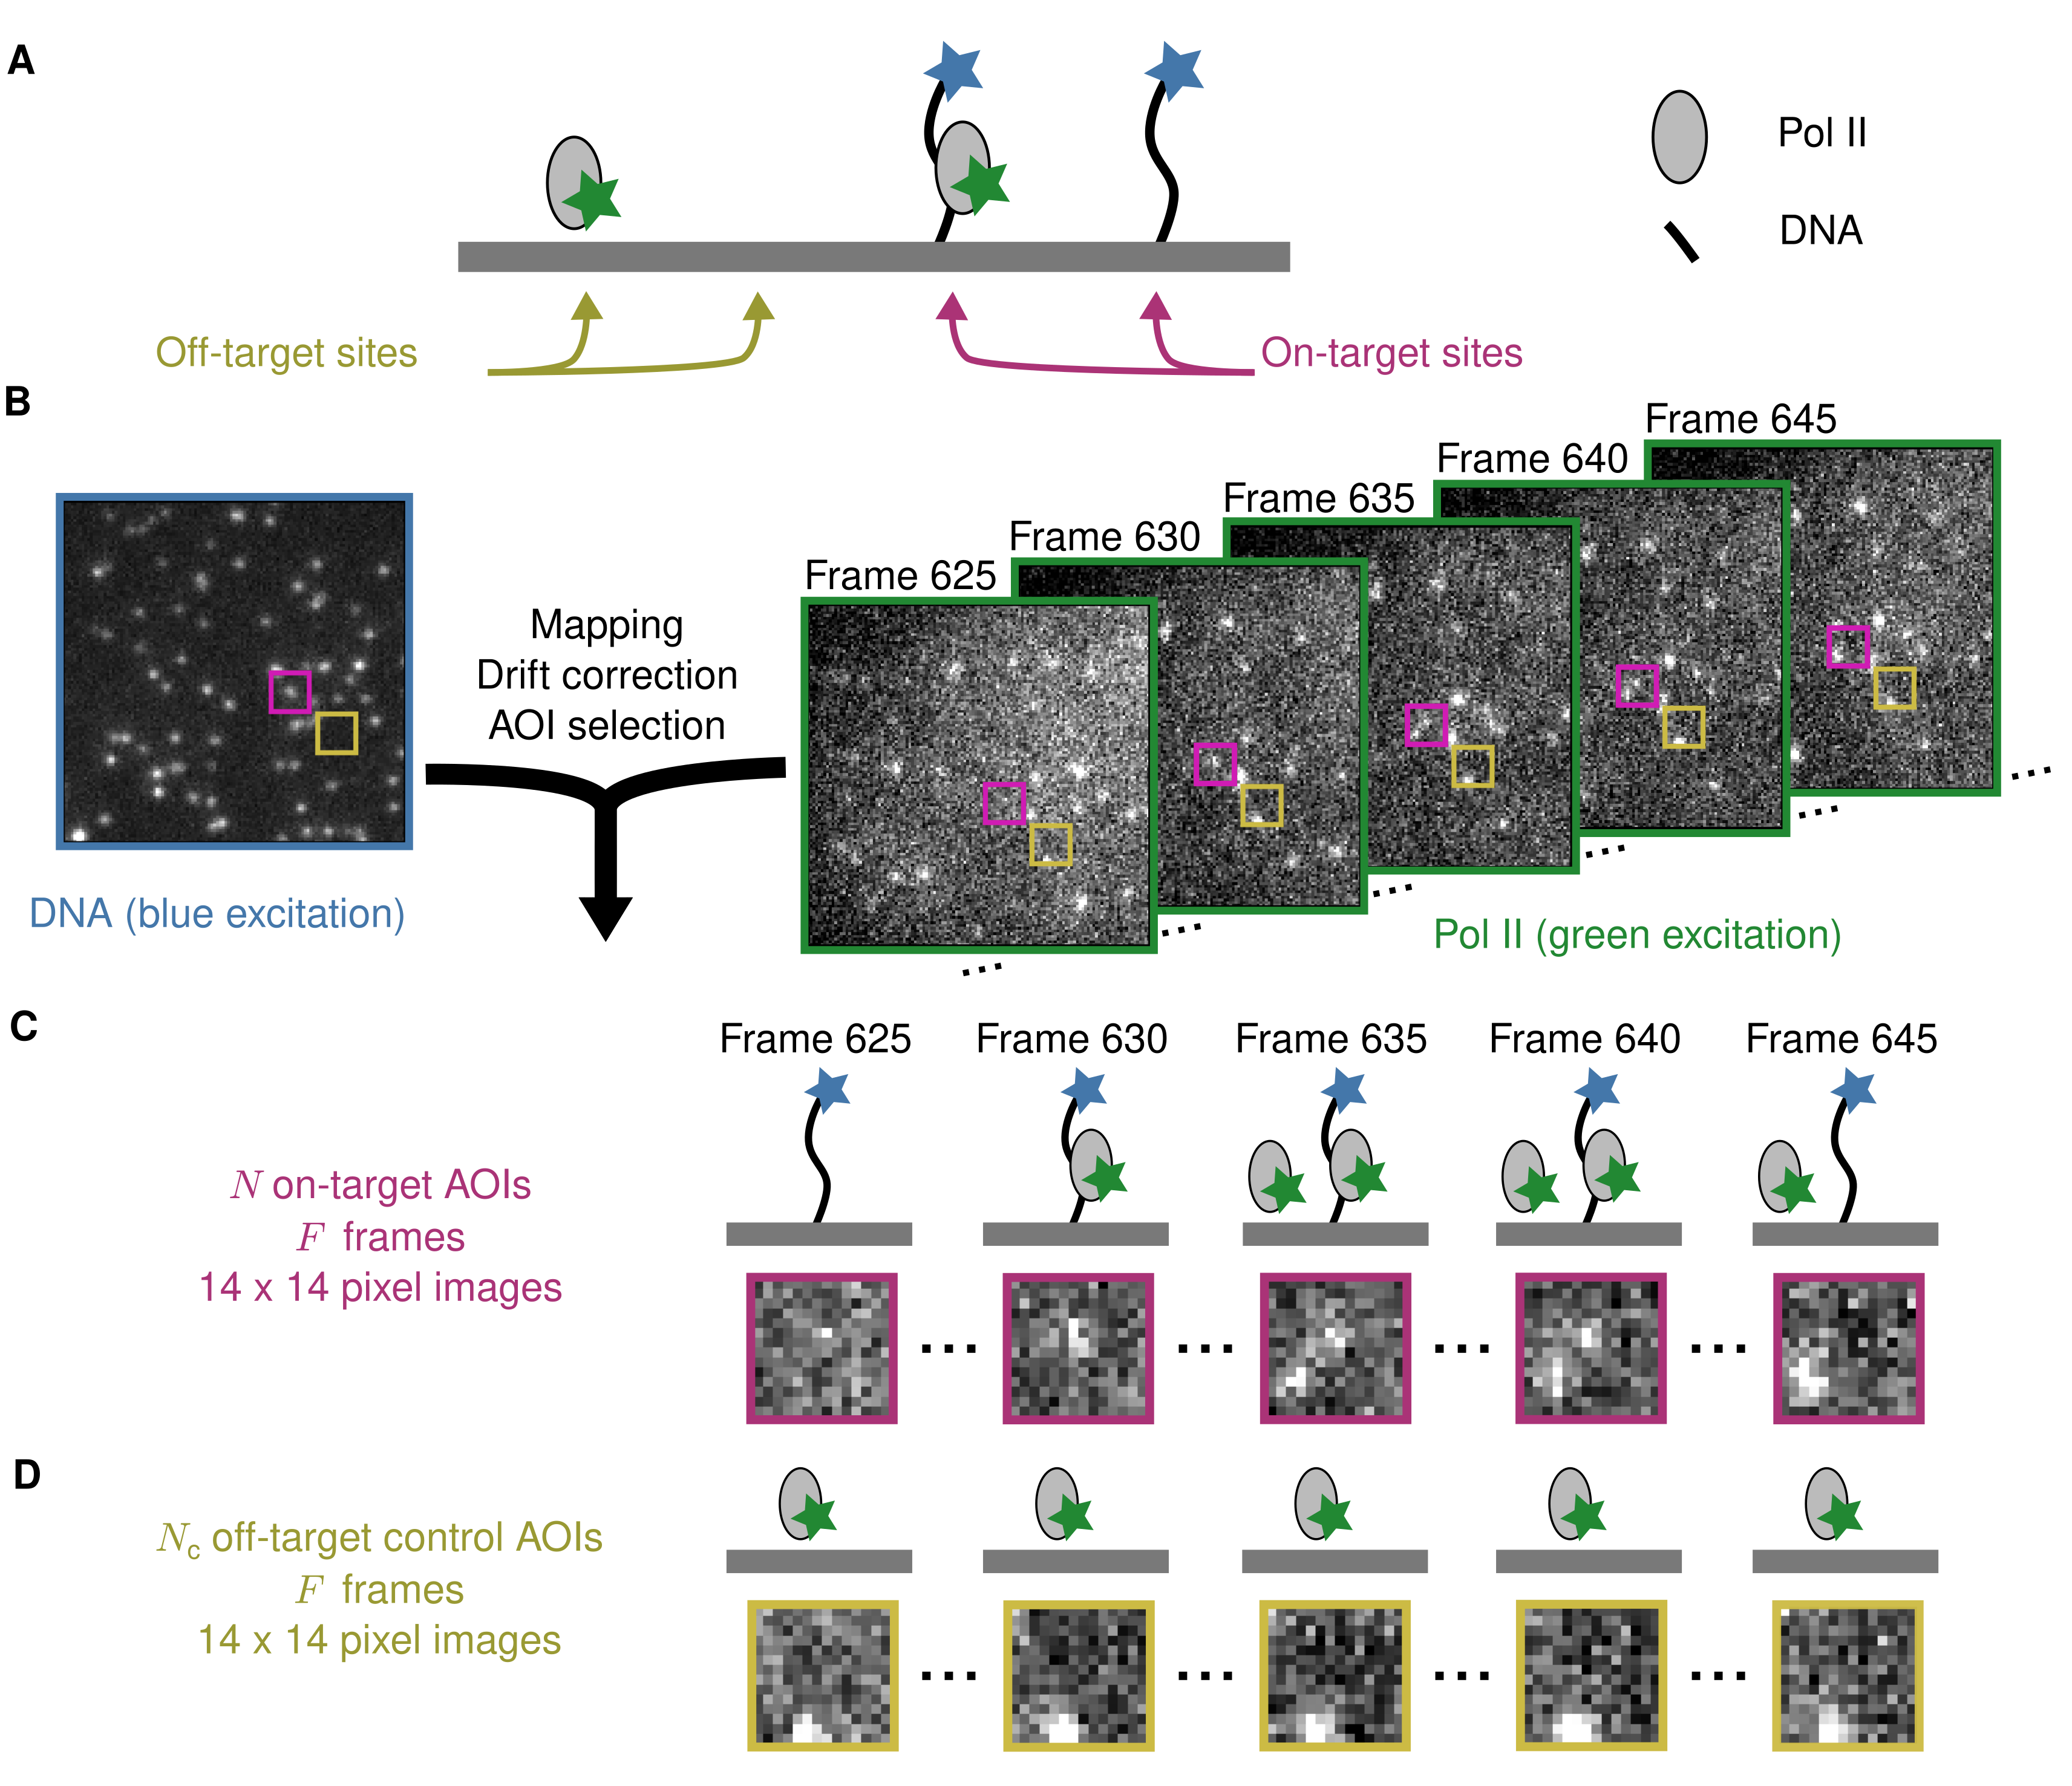
\includegraphics[width=145mm]{figures/cosmos_experiment/cosmos_experiment.png}
\caption{\textbf{Example CoSMoS experiment.} Data set A in \TABLE{datasets}. (\textbf{A}) Experiment schematic. DNA target molecules labeled with a blue-excited fluorescent dye (blue star) are tethered to the microscope slide surface. RNA polymerase II (Pol II) binder molecules labeled with a green-excited dye (green star) are present in solution. (\textbf{B}) Data collection and preprocessing. After collecting a single image with blue excitation to identify the location of the DNA molecules, a time sequence of Pol II images were collected with green excitation.  Preprocessing of the images includes mapping of the corresponding points in target and binder channels, drift correction, and identification of two sets of areas of interest (AOIs).  One set corresponds to locations of target molecules (e.g., purple square); the other corresponds to locations where no target is present (e.g., yellow square). (\textbf{C}) On-target data. Data are time sequences of 14 $\times$ 14 pixel AOI images centered at each target molecule. Frames show presence of on-target (e.g., frame 630) and off-target (e.g., frame 645) Pol II molecules. (\textbf{D}) Off-target control data. Control data consists of images collected from randomly selected sites at which no target molecule is present. }
\label{fig:cosmos_experiment}
\end{fullwidth}
\end{figure}

In this paper, we describe a qualitatively different Bayesian machine learning method for analysis of CoSMoS data implemented in a computer program, Tapqir (Kazakh: clever, inventive; pronunciation: \emph{tap-keer}). Tapqir analyzes two-dimensional image data, not integrated intensities.  Unlike prior methods, our approach is based on an explicit, global causal model for CoSMoS image formation and uses variational Bayesian inference \citep{Kinz-Thompson2021-tb,Gelman2013-ro} to determine the values of model parameters and their associated uncertainties. This model, which we call ``\emph{cosmos}'', implements time-independent analysis of single-channel (i.e., one-binder) data sets. The \emph{cosmos} model is physics-informed and includes realistic shot noise in fluorescent spots and background, camera noise, the size and shape of spots, and the presence of both target-specific and nonspecific binder molecules in the images. Most importantly, instead of yielding a binary spot-/no-spot determination, the algorithm calculates the probability of a target-specific spot being present at each time point and target location. The calculated probability can then be used in subsequent analyses of the molecular thermodynamics and kinetics. Unlike alternative approaches, Tapqir and \emph{cosmos} do not require subjective threshold settings so they can be used effectively and accurately by non-expert analysts. The program is implemented in the Python-based probabilistic programming language Pyro \citep{Bingham2019-qy}, which enables efficient use of graphics processing unit (GPU)-based hardware for rapid parallel processing of data and facilitates future modifications to the model.